\chapter{Optimisation and algorithms}
\section*{Routes and low-cost connectors}
A weighted graph assigns a number (such as distance, time or cost) to each edge. A shortest-path problem seeks a route of minimum total weight. In the Town Hall example, this means choosing a destination in the Blue Mountains and minimising the sum of the road-segment travel times. A minimum spanning tree (MST) seeks a least-total-weight set of edges connecting every vertex, without cycles. These are different questions: a shortest route between two points need not belong to every MST. The electricity-network example below is a deliberately simplified connectivity-and-cost model, not a design for the actual NSW grid.

\begin{figure}[htbp]
\centering
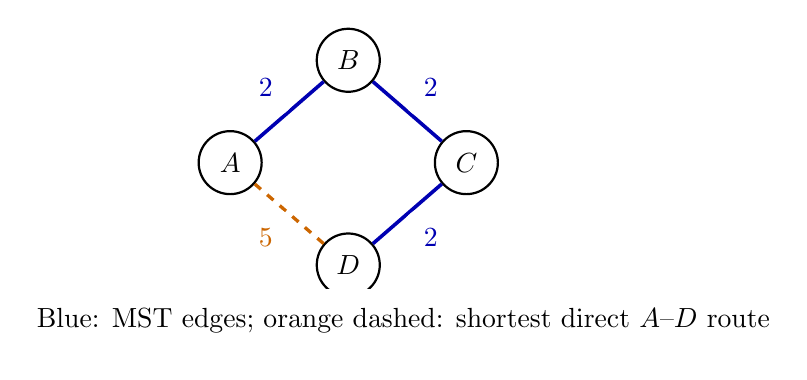
\begin{tikzpicture}[thick,every node/.style={circle,draw,fill=white,minimum size=8mm}]
\node (a) at (0,0) {$A$}; \node (b) at (1.5,1.3) {$B$}; \node (c) at (3,0) {$C$}; \node (d) at (1.5,-1.3) {$D$};
\draw[blue!70!black,line width=1.3pt] (a)--node[above left,draw=none,fill=white] {2} (b) (b)--node[above right,draw=none,fill=white] {2} (c) (c)--node[below right,draw=none,fill=white] {2} (d);
\draw[orange!80!black,dashed,line width=1.2pt] (d)--node[below left,draw=none,fill=white] {5} (a);
\node[draw=none,rectangle] at (2.2,-2) {Blue: MST edges; orange dashed: shortest direct $A$--$D$ route};
\end{tikzpicture}
\caption{The shortest route between two vertices and the minimum spanning tree solve different problems.}
\end{figure}

\section{A capacity-constrained delivery challenge}
\Challenge{} \Uni{} \textbf{Problem.} Suppose a town's two-way road network is a finite connected graph with positive road lengths. The inventory is at a vertex $O$, and there are $n$ delivery requests at vertices $P_1,\ldots,P_n$. Let $d$ denote shortest-path distance, let
\[
R=2\sum_{j=1}^n d(O,P_j)
\]
be the total distance for delivering every item separately, and let $W$ be the total length of all roads. A deliveryman can carry at most $k$ items per trip, where $k$ is a positive integer; every trip starts and ends at $O$. Prove that some delivery plan has total distance at most
\[
\frac{1}{k}R+\frac{2(k-1)}{k}W,
\]
and determine whether either coefficient can be decreased while the other is kept fixed.

\textbf{Solution.} First add requests at $O$ until the total number of requests is a multiple $km$ of $k$. These extra requests have zero travel cost and leave $R$ and $W$ unchanged, so removing them from any resulting plan gives a plan for the original requests with no greater distance. We may therefore work with $km$ requests.

Choose a shortest-path tree $T$ rooted at $O$. It is a subgraph of the road network, so its total length is at most $W$. Make a closed walk in $T$ that traverses each tree edge exactly twice, once in each direction. Its length is at most $2W$. List the requests $A_1,\ldots,A_{km}$ in the order their locations are first visited along this walk, listing requests at the same location consecutively, and put $A_{km+1}=A_1$. The shortest-path distance between consecutive locations is at most the length of the intervening part of the walk; for the final pair, use the end and beginning of the closed walk. Thus
\[
\sum_{i=1}^{km} d(A_i,A_{i+1})\leq 2W.
\]

For each of the $k$ cyclic shifts of this list, partition the requests into consecutive groups of $k$. Serve each group $A_i,\ldots,A_{i+k-1}$ on a trip that follows shortest paths from $O$ to $A_i$, between successive requests in the group, and from $A_{i+k-1}$ back to $O$. This is a feasible plan because the road network is undirected and each trip carries just its group's $k$ items.

Sum the lengths of all $k$ plans. Each request is the first in a group once and the last in a group once, so its radial path from and back to $O$ contributes $2d(O,A_i)$. The total radial contribution is therefore $R$. Each cyclic segment from $A_i$ to $A_{i+1}$ is internal to a group in $k-1$ shifts and is skipped at a group boundary in the other shift. The combined internal-segment contribution is at most
\[
(k-1)\sum_{i=1}^{km}d(A_i,A_{i+1})\leq 2(k-1)W.
\]
Hence the sum of the $k$ plan lengths is at most $R+2(k-1)W$. At least one plan has length no more than their average, giving the claimed bound.

Both coefficients are individually sharp. To see that $1/k$ cannot be lowered, fix $k$ and take a unit road $OX$, then attach $N=km$ distinct destinations to $X$ by separate spokes of length $\varepsilon=N^{-2}$. Then $W=1+N\varepsilon$, $R=2N(1+\varepsilon)$, and the optimal delivery distance $L_{\mathrm{opt}}$ is $2m+2N\varepsilon$: at least $m$ trips must each cross $OX$ out and back, and each short spoke must also be traversed twice. Grouping the destinations $k$ at a time attains this cost. As $m$ grows, $W$ stays near $1$, while $R/L_{\mathrm{opt}}\to k$. Thus any smaller coefficient of $R$, with the stated coefficient of $W$, eventually fails.

For the coefficient of $W$, take a star with centre $O$, $k$ unit-length spokes, and one request at the end of each spoke. Here $W=k$ and $R=2k$. Every spoke must be traversed twice, so the optimal total distance is $2k$. With the coefficient of $R$ fixed at $1/k$, any valid coefficient $\beta$ of $W$ must satisfy $2k\leq 2+\beta k$, or $\beta\geq 2(k-1)/k$. This includes $k=1$, when the sharp coefficient is $0$.

The averaging also explains the form of the bound: the total radial cost across the $k$ plans is always $R$, while the contribution from the closed tree walk is shared across those plans. For $k=1$ the bound is $R$; as capacity grows, it approaches the familiar tree-tour bound $2W$.

\section{Dijkstra's algorithm}
For a weighted graph with non-negative edge weights, Dijkstra's algorithm finds shortest-path distances from a chosen source $s$. It keeps a tentative distance $d(v)$ for each vertex and finalises these distances one at a time, from smallest to largest.

To find a shortest path from $s$ to a target $t$:
\begin{enumerate}
\item Set $d(s)=0$, set every other tentative distance to infinity, and leave all predecessor records empty.
\item Choose an unfinalised vertex $u$ with the smallest finite tentative distance and finalise it. If no such vertex remains, any unfinalised vertices are unreachable from $s$.
\item For each unfinalised neighbour $v$ of $u$, compare $d(u)+w(uv)$ with $d(v)$, where $w(uv)$ is the edge weight. If the new value is smaller, replace $d(v)$ with it and record $u$ as the predecessor of $v$.
\item Repeat until $t$ is finalised or no reachable unfinalised vertices remain. Follow predecessor records backwards from $t$ to recover the route.
\end{enumerate}

Here is a small illustrative model of the Town Hall question. The edge weights are illustrative travel times in minutes, not current route estimates. Let $H$ represent Town Hall, $M$ a chosen destination in the Blue Mountains, and $A,B$ intermediate road junctions. Starting at $H$, the algorithm first gives $A$ distance 2 and $B$ distance 5. After finalising $A$, it improves $B$ to 3 and gives $M$ distance 9. Finalising $B$ then improves $M$ to 5. Dijkstra's algorithm chooses $H$--$A$--$B$--$M$, with total time $2+1+2=5$ minutes; BFS chooses the two-edge route $H$--$B$--$M$, which takes $5+2=7$ minutes.

\begin{theorem}
Dijkstra's algorithm correctly computes shortest-path distances in a finite graph with non-negative edge weights.
\end{theorem}
\begin{figure}[htbp]
\centering
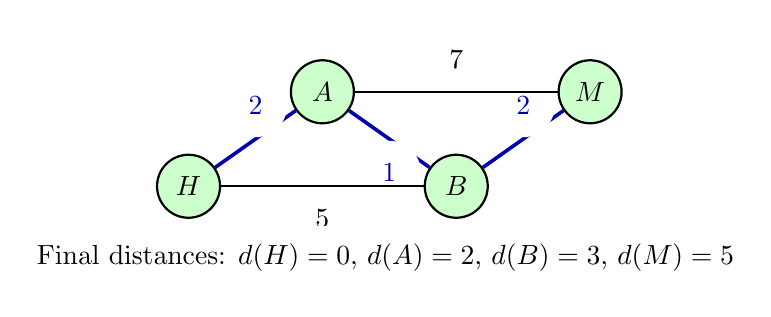
\begin{tikzpicture}[thick,every node/.style={circle,draw,fill=white,minimum size=8mm}]
\node[fill=green!20] (h) at (0,0) {$H$}; \node[fill=green!20] (a) at (1.7,1.2) {$A$};
\node[fill=green!20] (b) at (3.4,0) {$B$}; \node[fill=green!20] (m) at (5.1,1.2) {$M$};
\draw[blue!70!black,line width=1.3pt] (h)--node[above,draw=none,fill=white] {2} (a)--node[below,draw=none,fill=white] {1} (b)--node[above,draw=none,fill=white] {2} (m);
\draw (h)--node[below,draw=none,fill=white] {5} (b) (a)--node[above,draw=none,fill=white] {7} (m);
\node[draw=none,rectangle] at (2.5,-0.9) {Final distances: $d(H)=0$, $d(A)=2$, $d(B)=3$, $d(M)=5$};
\end{tikzpicture}
\caption{Illustrative travel times in minutes. $H$ is Town Hall, $M$ is a Blue Mountains destination, and $A,B$ are junctions.}
\end{figure}
\begin{proof}[Why the selection is safe]
Suppose $u$ is the unvisited vertex of smallest tentative distance. Any route to $u$ not already represented by a permanent vertex must reach some unvisited vertex first. The distance to that first unvisited vertex is at least the smallest tentative label, while the remaining edge weights are non-negative. Therefore no route through unvisited territory can reach $u$ with a smaller distance. So $u$'s label is final. Repeating this argument finalises every reachable vertex.
\end{proof}

Negative weights break the argument: a later route could reduce a distance after a vertex was marked permanent. For instance, an edge of weight $-5$ could make a route through an apparently longer intermediate vertex cheaper.

\section{Minimum spanning trees}
Kruskal's algorithm sorts edges from lightest to heaviest, adding an edge if it does not create a cycle. Prim's algorithm starts from one vertex and repeatedly adds a cheapest edge joining the current tree to a new vertex.

\begin{lemma}[Cut property]
For any cut (a partition of the vertices into two nonempty sets), a uniquely lightest edge crossing the cut belongs to every MST.
\end{lemma}
\begin{figure}[htbp]
\centering
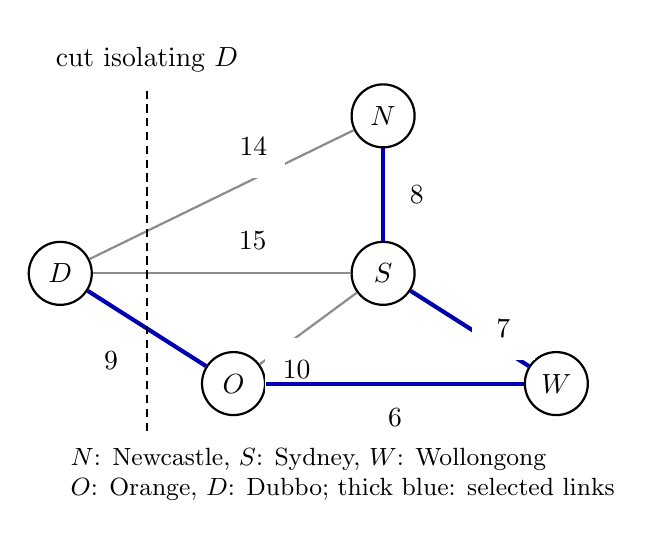
\begin{tikzpicture}[thick,every node/.style={circle,draw,fill=white,minimum size=8mm}]
\node (n) at (0.8,2) {$N$}; \node (s) at (0.8,0) {$S$};
\node (w) at (3,-1.4) {$W$}; \node (o) at (-1.1,-1.4) {$O$};
\node (d) at (-3.3,0) {$D$};
\draw[black!45] (d)--node[pos=.62,above,rectangle,text=black,draw=none,fill=white] {14} (n);
\draw[black!45] (s)--node[pos=.62,below,rectangle,text=black,draw=none,fill=white] {10} (o);
\draw[black!45] (d)--node[pos=.62,above,rectangle,text=black,draw=none,fill=white] {15} (s);
\draw[blue!70!black,line width=1.5pt] (o)--node[below,rectangle,text=black,draw=none,fill=white] {6} (w);
\draw[blue!70!black,line width=1.5pt] (s)--node[pos=.5,right,rectangle,text=black,draw=none,fill=white] {7} (w);
\draw[blue!70!black,line width=1.5pt] (s)--node[right,rectangle,text=black,draw=none,fill=white] {8} (n);
\draw[blue!70!black,line width=1.5pt] (d)--node[pos=.48,below left,rectangle,text=black,draw=none,fill=white] {9} (o);
\draw[black,densely dashed] (-2.2,-2.0)--(-2.2,2.55);
\node[draw=none,rectangle,fill=white] at (-2.2,2.72) {cut isolating $D$};
\node[draw=none,rectangle,align=left,anchor=west,font=\small] at (-3.3,-2.55) {$N$: Newcastle, $S$: Sydney, $W$: Wollongong\\$O$: Orange, $D$: Dubbo; thick blue: selected links};
\end{tikzpicture}
\caption{A fictional NSW-inspired network. Edge labels are invented cost units, and the schematic locations and links are not actual transmission routes.}
\label{fig:nsw-mst-model}
\end{figure}
\begin{proof}
If an MST omitted that edge, add it. This creates a cycle, which must contain another edge crossing the same cut. Removing that other, heavier edge leaves a spanning tree of smaller total weight, contradicting minimality.
\end{proof}

\begin{example}[A simplified electricity-link model]
Suppose the five labelled hubs and candidate links have the invented costs shown in Figure~\ref{fig:nsw-mst-model}. Kruskal accepts $OW=6$, $SW=7$, $SN=8$, and $OD=9$, connecting all five hubs with four links and total cost $30$. The cut isolating Dubbo is crossed by $OD=9$, $ND=14$, and $SD=15$. Since $OD$ is uniquely cheapest, the cut property guarantees that every MST contains it.
\end{example}

The tree selected above is the path $D$--$O$--$W$--$S$--$N$. If the design also requires protection from any one link failure, adding the candidate link $ND=14$ closes a cycle through all five hubs. The resulting five-link network costs $30+14=44$ and remains connected after deleting any one of those five links. This illustrates how a resilience requirement changes the optimisation question.

\Enrichment{} \textbf{Why Kruskal's algorithm works.} Adding an edge $e$ not in a spanning tree $T$ creates a cycle. Removing any other edge $f$ on that cycle gives another spanning tree, $T-f+e$; this is the edge-exchange lemma.

\begin{proof}[Correctness of Kruskal's algorithm]
The selected edges always form a forest. Since the original graph is connected, whenever this forest has more than one component there is an edge joining two of them; Kruskal eventually considers and accepts such an edge. Thus the algorithm ends with a spanning tree.

To see that it has minimum weight, start with any minimum spanning tree $T$ containing all edges Kruskal has selected so far; initially, any minimum spanning tree works. Let $e$ be the next edge selected. If $e$ is already in $T$, keep $T$. Otherwise, adding $e$ to $T$ creates a cycle. Since $e$ joins distinct components of the selected forest, that cycle contains another edge $f$ crossing the cut between the component containing one endpoint of $e$ and the rest. Every edge crossing this cut is eligible for addition to the selected forest, so Kruskal's choice gives $w(e)\leq w(f)$. Replacing $f$ by $e$ gives a spanning tree of no greater weight, hence another minimum spanning tree containing the longer selected prefix. Repeating proves that Kruskal's final tree is minimum.
\end{proof}

\Enrichment{} If all edge weights are distinct, the minimum spanning tree is unique. At each step, the next Kruskal edge is the uniquely lightest edge crossing the cut between one current forest component and the rest. By the cut property, every minimum spanning tree must contain it. This holds at every step, so every minimum spanning tree is Kruskal's tree.

\section{How algorithms scale}
An algorithm's input size grows with the number of vertices and edges. A method taking roughly $n^2$ elementary steps may be practical for hundreds or thousands of objects, while one taking roughly $2^n$ steps quickly becomes infeasible. This qualitative comparison is more useful than timing one small example on one computer.

\section*{Exercises}
\begin{enumerate}
\item Run Dijkstra's algorithm on a small weighted graph of your choice. Show each tentative-distance update.
\item Construct a graph with a negative edge for which Dijkstra's algorithm finalises an incorrect distance.
\item On the five-hub model in Figure~\ref{fig:nsw-mst-model}, run Prim's algorithm starting at Sydney and run Kruskal's algorithm. List the accepted links in order and find the total cost of the MST.
\item Explain why the cut property justifies a cheapest edge across a cut in an MST, but does not justify choosing each next edge greedily when constructing a travelling-salesperson tour.
\end{enumerate}
